\documentclass[../main.tex]{subfiles}


\begin{document}

\section{MCMC simulation of a single chain in a spherical micelle}

Markov Chain Monte Carlo (MCMC) simulations can be used to sample a statistical ensemble (usually the Boltzmann ensemble).
In a MCMC simulation one proposes simulation step -- which is usually a small local change -- that than is either accepted or rejected.
The acceptance rate can be chosen in a few different ways, but the one most commonly used is the so-called Metropolis acceptance rate.
The Metropolis acceptance rate $\alpha$ of a proposed step from configuration $\left\{ r \right\} i$ to configuration $\left\{ r \right\} j$ is given by 
\[
    \alpha = \text{min}\left( 1, \exp( \beta (H(\left\{ r \right\}_i) - H\left\{ r \right\} _j) )\right)
.\] 
It is directly connected to another important concept: The concept of detailed balance.
The MCMC simulation fulfills detailed balance if 
\[
    P(\left\{ r \right\}_i) = 
    \frac{
        t(\left\{ r \right\}_j | \left\{ r \right\}_i)
    }{
        t(\left\{ r \right\}_i | \left\{ r \right\}_j)
    }
    P(\left\{ r \right\}_j)
,\] 
where $t(\left\{ r \right\}_j | \left\{ r \right\}_i)$ is the probability to transition from state $i$ to state $j$.
Choosing the acceptance rate in the Boltzmann ensemble like above ensures that this holds.
The acceptance rate is probed numerically by proposing a random number between zero and one.
If the proposed number is smaller than $\alpha$ the step is accepted, otherwise rejected.
\par

In this project we look at the ensemble of a polymer mad up of two sub chains. 
The polymer is embedded in two external fields -- where one chain of the polymer interacts with only one field, respectively.
This description has been derived from a collection of copolymers where the same sub chains are attracting each other while opposite sub chains are repelling one another.
Collectively the copolymers form a micelle, where the shorter sub chains are on the inside.
Ultimately we want to find the escape rate for a single copolymer to leave the micelle using MCMC techniques.


\subsection{Homopolymer simulations}

\subsubsection{End-to-End vector}

\begin{figure}[htpb]
    \centering
    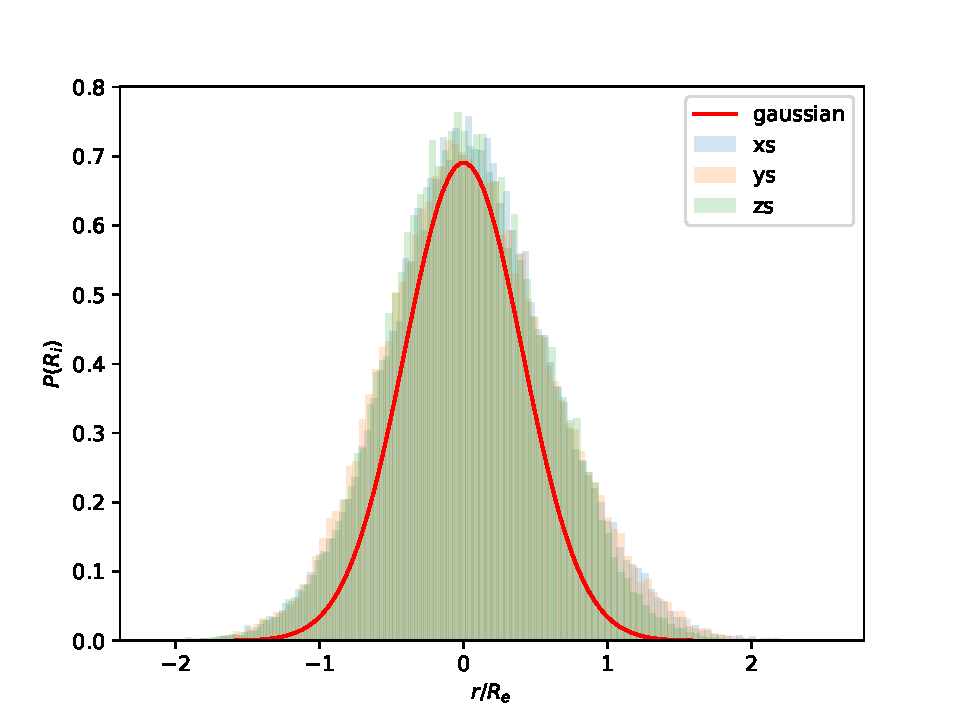
\includegraphics[width=0.8\textwidth]{../figures/ex1_end_to_end_homopolymer.pdf}
    \caption{
        Distribution of coordinate components for the end-to-end vector of the free homopolymer obtained from a MCMC simulation.
        The simulation was executed for a total of \num{e6} sweeps -- discarding the first \num{e5} to ensure equilibrium dynamics.
    }
    \label{fig:ex1_end_to_end_homopolymer}
\end{figure}

To ensure that the result of our MCMC simulation is correct we verify it by looking at the case without any external fields (the case of a homopolymer).
About this system we can make exact predictions from the Rouse-Model that we can use to verify our simulation technique.
The Rouse-Model makes predictions about the distribution of the end-to-end vector $\mathbf{R}$ of the polymer (distance between first and last beed of the polymer).
Specifically, it predicts that the distribution is gaussian with $\left< \mathbf{R} \right> = \mathbf{0}$ and $\left< \mathbf{R} \right> = \unit{\charlength\squared}$.
\par

In Figure \ref{fig:ex1_end_to_end_homopolymer} we can see the overlayed distributions of the components of $\mathbf{R}$.
We can clearly see that the distribution has very gaussian-like features and the means of the individual components x/y/z (\qtylist{.0574; .0446; .0263}{\charlength}) also correspond correctly to the predictions of the Rouse-Model.
From the rules of gaussian error propagation we can see that summing the individual variances of components yields the total variance of $\mathbf{R} ^2$.
Such, looking at the variances of the individual components (\qtylist{.3225;.3359;.2915}{\charlength\squared}) we can also verify that the prediction for $\left<\mathbf{R} ^2 \right>$ holds.


\subsubsection{Mean Square Deviation and Diffusion}

\begin{figure}[htpb]
    \centering
    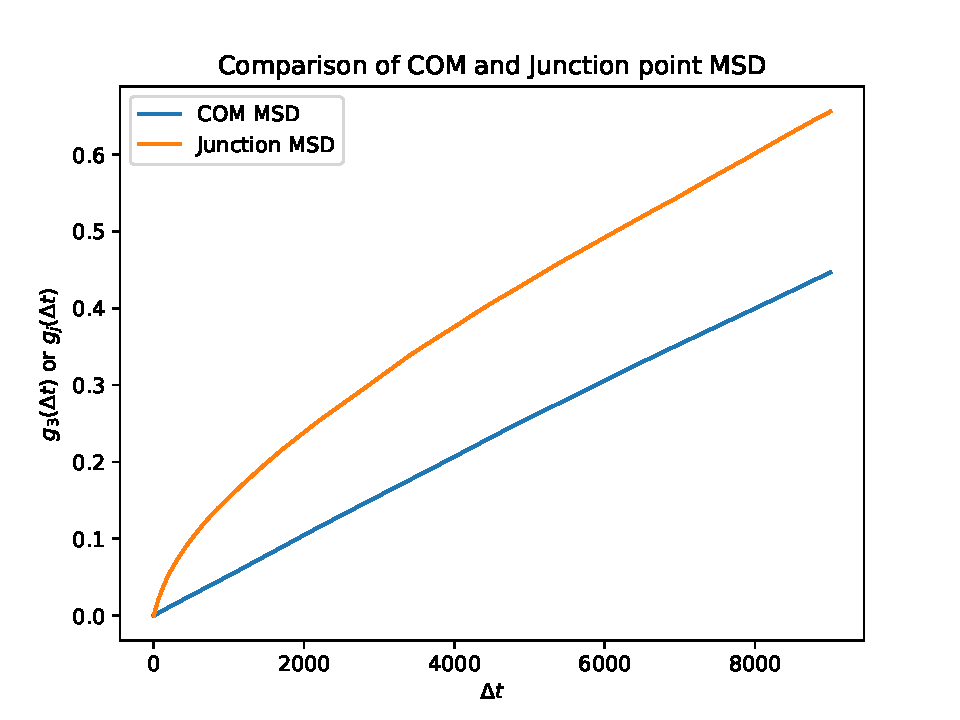
\includegraphics[width=0.8\textwidth]{../figures/ex1_msd_comparison.pdf}
    \caption{
        Comparison of the MSD of the COM and the MSD of the junction point of a homopolymer.
        COM/junction point MSD ($g_r$/$g_j$) is plotted against the difference in time measured in MC sweeps.
        Simulation data was obtained from the same simulation as in Figure \ref{fig:ex1_end_to_end_homopolymer}.
    }
    \label{fig:ex1_msd_comparison}
\end{figure}

Another property we can investigate in the homopolymer is it's self-diffusion behavior.
For this we can calculate the Mean Square Deviation (MSD) of the Center of Mass (COM) of the homopolymer.
Alternatively we can also calculate the MSD of the junction point which we define as the middle between the connected beeds of the subchains of a copolymer.
Note we are still dealing with the homopolymer here, but we take the junction point such that it corresponds to the same point in the homopolymer.
\par

Both MSDs are plotted in Figure \ref{fig:ex1_msd_comparison}.
We can clearly see that the MSD of both points in the chain asymptotically approach linear growth (also see the linear regressions in the attached jupyter notebook).
While we can see that the MSD of the junction point is generally larger than the MSD of the COM, both asymptotically show the same rate of growth.
This rate of growth is connected to the self-diffusion coeffecient.
\par

To calculate this self-diffusion coefficient we can either use 
\[
    D = \lim\limits_{\Delta t \to \infty} g(\Delta t)/6\Delta t
,\] 
or we make a linear fit to get the slope of the asymptote.
Doing so we obtain $D = \SI{8.6e-6}{\charlength\squared\per\mcstep}$.


\subsection{Copolymer simulations}

\begin{figure}[htpb]
    \centering
    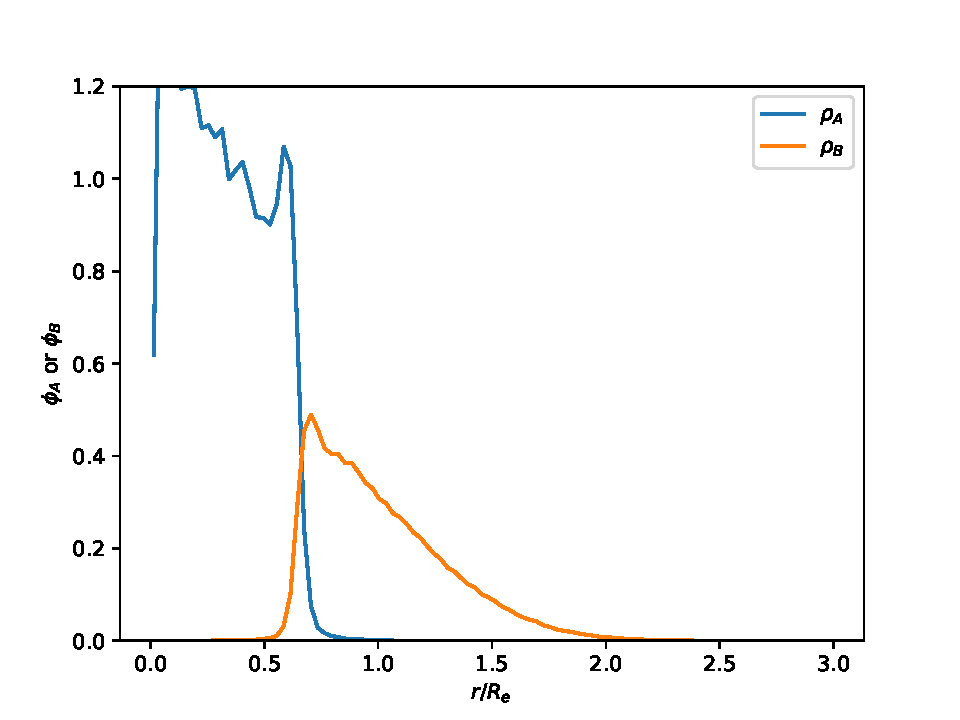
\includegraphics[width=0.8\textwidth]{../figures/ex1_partial_density_profile.pdf}
    \caption{
        Partial density profile of the two sub chains of the polymer plotted against the radius.
        Simulations were executed over \num{e6} MC sweeps while the first \num{e5} were discarded.
        The configuration's segments were weighted as if we were only looking at a singular thread leaving the micelle.  
    }
    \label{fig:ex1_partial_density_profile}
\end{figure}

To verify the correctness of the simulation of a copolymer (external fields switched on) we compare the radial partial density profile of the sub chains with the results obtained from self-consistent mean-field theory given on the exercise sheet.
In Figure \ref{fig:ex1_partial_density_profile} we can see the calculated result for the density profile.
Note that the domain around $\nicefrac{r}{R_e} = 0$ for the $A$ sub chain is quite ragged because of the radial nature of the plot.
As we approach small radii the sampled volume at each bin in the density becomes very small and we don't achieve the necessary accuracy to obtain the correct value for $\phi_A(0)$ (which is 1).
\par

\subsection{Free Energy from Umbrella potential}

To calculate the Free Energy landscape of the system we first need to do some analytical preparation.
We can add an umbrella potential to the Hamiltonian of our system to sample the system at a particular point in our landscape.
Afterwards we can remove that umbrella potential again from the correct value of the Free Energy to obtain the correct local values for the Free Energy. 
\par

To do so we calculate 
\begin{align*}
    \dv[]{F}{r} &= \dv[]{}{r} 
    \lim\limits_{k \to \infty} 
    -\frac{1}{\beta} 
    \ln 
    \sum\limits_{\left\{ \mathbf{r}_i \right\} }^{} 
    \sqrt{\frac{k}{2 \pi R_e^2}} 
    \exp( -  \beta\mathcal{H}(\left\{ \mathbf{r} _i \right\} | r ) ) \\
    &= 
    -\frac{1}{\beta} 
    \lim\limits_{k \to \infty}
    \frac{
        \sqrt{\frac{k}{2 \pi R_e^2}} 
        \dv[]{}{r} 
        \sum\limits_{\left\{ \mathbf{r}_i \right\} }^{} 
        \exp( -  \beta\mathcal{H}(\left\{ \mathbf{r} _i \right\} | r ) )
    }{
        \sum\limits_{\left\{ \mathbf{r}_i \right\} }^{} 
        \sqrt{\frac{k}{2 \pi R_e^2}} 
        \exp( -  \beta\mathcal{H}(\left\{ \mathbf{r} _i \right\} | r ) )
    }
    \\
    &= 
    -\frac{1}{\beta} 
    \lim\limits_{k \to \infty}
    \frac{
        \sum\limits_{\left\{ \mathbf{r}_i \right\} }^{} 
        - \beta\mathcal{H}(\left\{ \mathbf{r} _i \right\} | r )
        \exp( -  \beta\mathcal{H}(\left\{ \mathbf{r} _i \right\} | r ) )
    }{
        Z_k
    }
    \\
    &= 
    \left< 
    \pdv[]{
        \mathcal{H}(\left\{ \mathbf{r} _i \right\} | r )
    }{r} 
    \right>_k
    \\
.\end{align*}

But we also know 

\[
    \pdv[]{
        \mathcal{H}(\left\{ \mathbf{r} _i \right\} | r )
    }{r} 
    = 
    \pdv[]{}{r} \left( 
        -k \frac{k_B T}{2R_e^2} (r- r_j)^2
    \right) )
    = 
    -k \frac{k_B T}{R_e^2} (r- r_j)
.\] 

This we can use to calculate the local free energies by numerically integrating $\dv[]{F}{r} $.


\subsection{Free Energy Barrier}

\begin{figure}[htpb]
    \centering
    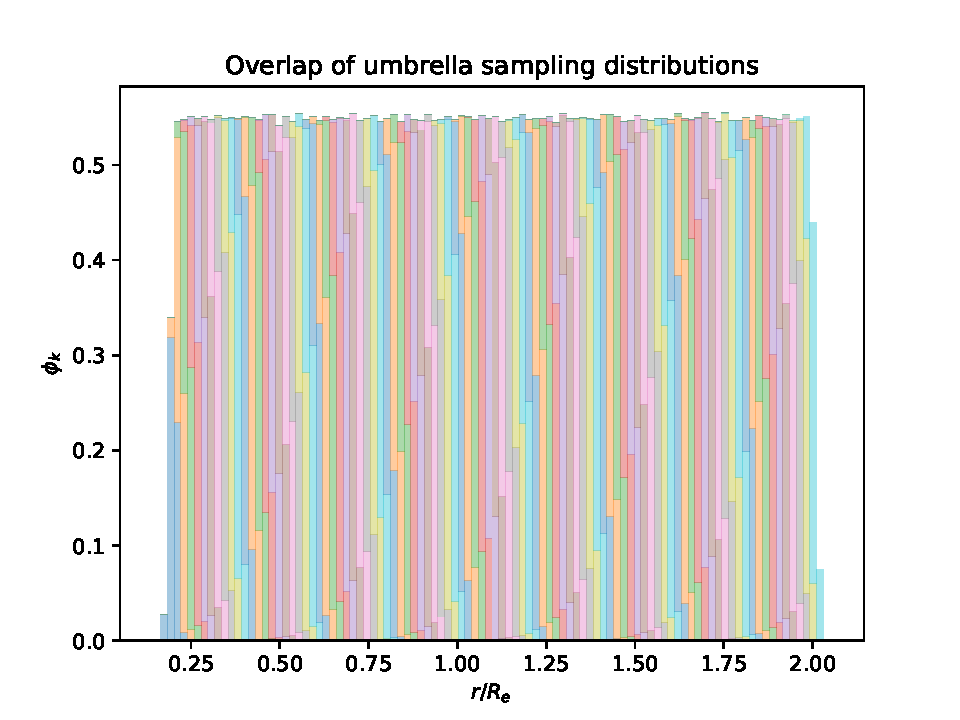
\includegraphics[width=0.8\textwidth]{../figures/ex1_overlap_umbrella.pdf}
    \caption{
        In this graphic we show that our grid of umbrella ensembles generate overlapping distributions in the junction point $r_j$.
        Every color corresponds to an independent umbrella ensemble run for \num{e6} MC sweeps, discarding the first \num{e5}.
        The constraint for the individual ensembles varies in steps of \SI{2e-2}{\charlength} from \qtyrange{.2}{2}{\charlength} and shown are \num{90} distributions in total.
    }
    \label{fig:ex1_overlap_umbrella}
\end{figure}

\begin{figure}[htpb]
    \centering
    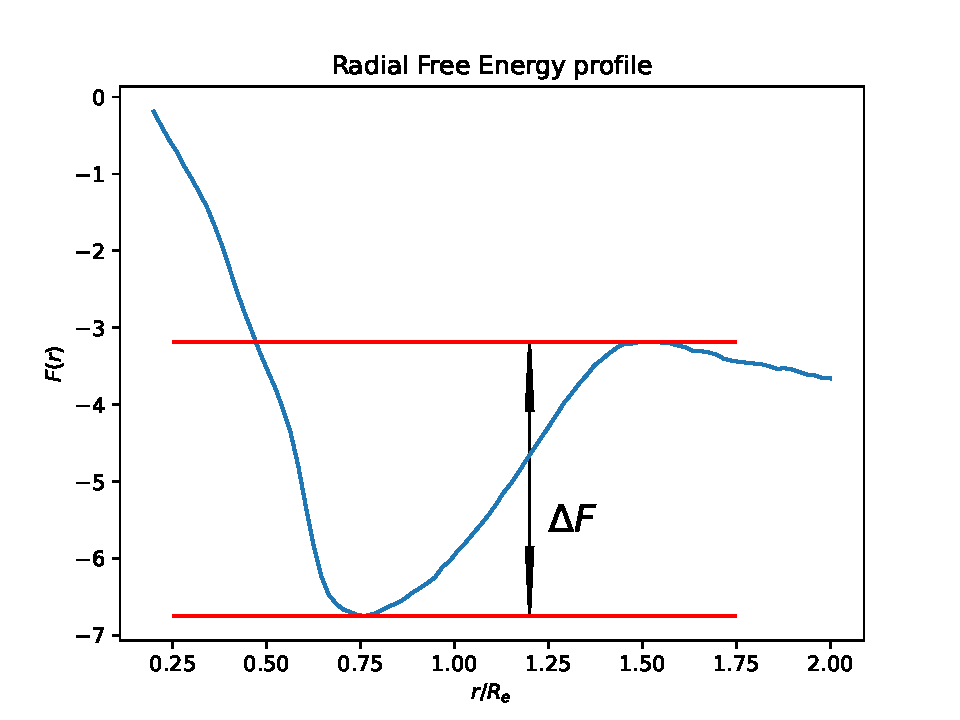
\includegraphics[width=0.8\textwidth]{../figures/ex1_free_energy_profile.pdf}
    \caption{
        Free Energy profile calculated from the umbrella sampling plotted against the junction point of the copolymer.
        The bottom of the basin and the top of the barrier are marked by horizontal red lines.
        $\Delta F$ as the difference between these lines is \SI{3.56}{\charenergy}.
    }
    \label{fig:ex1_free_energy_profile}
\end{figure}

To calculate the free energy profile of the system we can use -- as mentioned in the section above -- the umbrella sampling at different locations along a suitable reaction coordinate.
That suitable reaction coordinate in our case is the junction point of the copolymer.
From the results of the previous section we know that we can calculate the Free energy via the values of the junction point in the umbrella ensemble.
\par

Firstly we need to show that the grid we used for the umbrella sampling is sufficiently small, s.~t.~the local free energy does not vary too much from site to site on the grid.
We can achieve this by checking that the umbrella ensembles generate overlapping distributions in the reaction coordinate.
In Figure \ref{fig:ex1_overlap_umbrella} we can clearly see, that this is the case for our experiment.
\par

Now we can use the umbrella ensembles to calculate the local Free Energy along the reaction coordinate using the formula derived earlier.
In Figure \ref{fig:ex1_free_energy_profile} we can see the results of these calculations.
In the figure the height of the barrier is already marked.
It is $\Delta F = \SI{3.56}{\charenergy}$.


\ifSubfilesClassLoaded{
	% if it's compiled alone
}{
	% if it's compiled in the main file
    \newpage
}
\end{document}
